%%%%%%%%%%%%%%%%%%%%%%%%%%%%%%%%%%%%%%%%%%%%%%%%%%%%%%%%%%%%%%%%%%%%%%%%%%%%%%%%%%%%%%%%%%%%%%%%%%%%%%
%
%   Filename    : chapter_1.tex 
%
%   Description : This file will contain your Research Description.
%                 
%%%%%%%%%%%%%%%%%%%%%%%%%%%%%%%%%%%%%%%%%%%%%%%%%%%%%%%%%%%%%%%%%%%%%%%%%%%%%%%%%%%%%%%%%%%%%%%%%%%%%%

\chapter{Introduction}
\label{sec:intro}    %--note: labels help you with hyperlink editing (using your IDE)

Social media platforms have been used as means of self-expression for users. These platforms give users the possibility to express and expose their identity \citep{Marcus2006}. As such, data from social media platforms can lead us to gain insights from personality traits of these users. 

%%This chapter builds the motivation for the conduct of the research through a description of the background of the study or the current state of technology. This is followed by the research objectives, the scope and limitations, and significance of the research. The chapter ends with the research methodology describing the different activities to be conducted to achieve the goals of this research.%%


%%
%% --- 1.1 Background of the Study --- %%
%%

\section{Background of the Study}
\label{sec:overview}

%
%   NOTE: You have to delete/replace the unnecessary paragraphs with your own text.
%


%%This section gives the reader an overview of the specific technology or field in the international or local setting. The information regarding the technology or field should be contemporary and not
%%based on outdated sources. Discussion must not be too technical or too detailed.

%%Follow the inverted pyramid to describe each of the following. Allocate one (1) paragraph per level in the pyramid. 

% Describe the research area
Personality is defined as “patterns of thought, emotion, and behavior” \citep{Vinciarelli2014}. In a society, people develop opinions and treat each other differently based on their perception of the person’s personality. Understanding personality plays a significant role in fields such as psychology as this information can be used in studies of mental health and human behavior. Alongside the rise of publicly available and easily accessible information on social networking sites (SNS), the field of personality computing has begun to garner increasing interest in the last few years. 

%Research area ...
%This study's main research area is on personality computing. Personality computing is related to artificial intelligence and personality psychology by studying one's personality through a variety of computational techniques from different sources (usually text, multimedia, and social networks). Among the three main problems personality computing addresses; automatic personality recognition, perception, and synthesis \citep[p.~280]{Vinciarelli2014}; this study focuses on automatic personality recognition.
Personality computing integrates artificial intelligence and personality psychology by analyzing personality traits using a variety of computational techniques from various data sources, such as text, multimedia, and social networks. In this area of study, personality often represented as quantifiable traits, with the Big Five Personality model being a widely used framework. The Big Five model categorizes personality into five traits, namely: extraversion, agreeableness, conscientiousness neuroticism, and openness. 

Personality computing research is commonly divided into three subfields: Automatic Personality Recognition (APR), Automatic Personality Perception (APP), and Automatic Personality Synthesis (APS) \citep{Vinciarelli2014}.

% Describe the domain (where will you apply the topic)
Automatic personality recognition (APR) aims to infer the personality of an individual based on their digital footprint. APR has been traced back to the work of \citet{Pennebaker1999} wherein they asked the question of \textit{can language use reflect personality style?}

% Give a synthesis of previous work

% Synthesis of previous studies...
%\citet{Pennebaker1999} and \citet{Mairesse2007} had demonstrated the different ways of detecting personalities and emotions by analyzing the text with various language models. Due to that, social media had became a common place for the research of personality detection. The PagkataoKo dataset has been made with social media activity on Instagram and X (formerly known as Twitter). There were more studies using X's data than Instagram due to X being a more prominent platform with its text-based posts. However, \citet{ferwerda2016}, \cite{Reece2017-qw} and \cite{Harris2019-gq} made studies that showed analyzing photos was possible. Thus, researching on Instagram became more meaningful in this manner.
Previous studies have found success in the implementation of deep learning and deep neural networks in the field of APR \citep{Zhao2022}. The standard approach involves feature extraction, followed by machine learning techniques to associate extracted features with personality traits. Common models include deep neural networks (DNNs) and support vector machines (SVMs). 

The widespread adoption of social media has further propelled APR research, providing large-scale, real-time behavioral data for personality inference. Studies suggest that social media interactions exhibit behavior that is “spontaneous and self-disclosing beyond intention” \citep{Vinciarelli2014}, making them valuable for personality analysis. Thus, many studies have taken to conducting personality analysis using data from personal social media profiles. Text was a common modality in their research, though a smaller number of papers have also explored image-based analysis. 

Despite growing research in APR, most studies have primarily focused on Western populations. Limited research has explored personality inference methods within Filipino contexts, particularly in using image-based data.

% State the problem and the research question

% Paragraph containing the Problem Statement or the Research Question.

This study seeks to explore image-based APR methods tailored for Filipino users by leveraging Instagram data, integrating psychological analysis and computational techniques. The study aims to address the question: \textit{How can Instagram content, including images and captions, be used to infer a Filipino’s personality traits based on psychological and computational analysis?}

% This section ends with a discussion on the problem/s faced by or that still exist in the specific technology or field (e.g., limitations of existing software or algorithms). It should not contain your research objectives or goal; instead, the problem statement would lead to the research objectives to be stated in 1.2.

% \subsection{Figures}

% Often times, a graph, illustration, screenshot, or any image can help a reader better understand what we say in text. In academic writing, we call them \textbf{figures}. Please add as many figures as necessary to help build your narrative, but do not go overboard. 

% You can add figures in JPG or PNG format as shown in Figure \ref{fig:disneystock}. All figures should also have a descriptive caption. As a general principle, your caption should adequately describe what is shown in the figure, and not just short texts. If we remove all the surrounding text, the reader should still understand what your figure is. 

% All figures should be referred to at least once in the surrounding paragraphs. Make sure that you explain what the figure is all about, and that you refer to your figure. You can also use the surround paragraphs to highlight key insights or parts of your figure. For example, \figref{fig:disneystock} shows a graph of the performance of Disney stock from the 1980s to 2012.

% %--- the following example shows how to include a figure in PNG format
% \begin{figure}[t]                %-- use [t] to place figure at top, [b] to place at the bottom, [h] for here
%    \centering                    %-- use this to center the figure
%    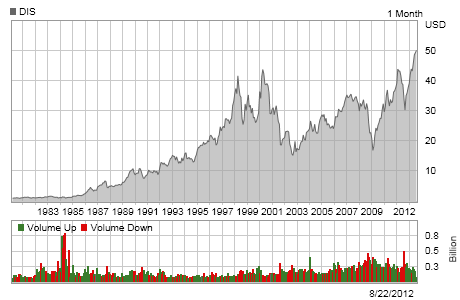
\includegraphics{DisneyChart.png}      %-- include image file named as "disneychart.png" 
%    \caption{Disney's stock price chart from the 1980s up to 2012. The top chart shows the stock price in each month. The bottom chart shows the change in volume of transactions. The bars are colored based on the type of movement that happened in a month.}
%     \label{fig:disneystock}
% \end{figure}

% \subsection{References}

% Some notes on citing references. When using APA format, the author-date method of citation is followed. This means that the author's last name and the year of publication for the source should appear in the text, and a complete reference should appear in the reference list.

% %
% % Examples:
% %     	Smith (1970) compared reaction times . . .
% %     	In a recent study of reaction times (Smith, 1970), . . .   
% %     	In 1970, Smith compared reaction times . . .
% %	Smith, et al., (1970) compared reaction times . . .
% %     	In a recent study of reaction times (Smith, et al., 1970), . . .  
% %     	In 1970, Smith, et al., compared reaction times . . .
% %

% Here are some examples on how to do the referencing (note author's name and years are different from commented examples). For APA citation details, refer
% to \url{http://www.ctan.org/tex-archive/biblio/bibtex/contrib/apacite/}. 

% \begin{itemize}
%  \item \citeA{kartch:2000:ERA} compared reaction times...
%  \item In a recent study of reaction times \cite{kartch:2000:ERA}...
%  \item In \citeyearNP{kartch:2000:ERA}, \citeauthor{kartch:2000:ERA} compared reaction times...
%  \item \shortciteA{fedkiw:2001:VSO} compared reaction times... 
%  \item In a recent study of reaction times \cite{fedkiw:2001:VSO}...
%  \item In \citeyearNP{fedkiw:2001:VSO}, \shortciteauthor{fedkiw:2001:VSO}, compared reaction times...
% \end{itemize}

% The following are references from journal articles \cite{Park:2006:DSI, Pellacini:2005:LAH, sako:2001:SSB}.  Here's an MS thesis document \cite{yee:2000:SSA}, and this is from a PhD dissertation \cite{kartch:2000:ERA}. For a book, reference is given as \cite{parke:1996:CFA}.  Proceedings from a conference samples are \cite{Jobs95, fedkiw:2001:VSO,levoy:2000:TDM}.  

% The sample bibliography file named \textbf{myreferences.bib} is from the
% SIGGRAPH \LaTeX template.  You can use a text editor to view the contents of the bib file. It is your task to create your own bibliography file.  For those who downloaded papers from ACM or IEEE sites, there is a BibTeX link that you can click; thereafter, you just simply need to copy and paste the BibTeX entry into your own bibliography file.

% \subsection{Code snippet}

% The following shows how to include a program source code (or algorithm). The verbatim environment, as the name suggests, outputs text (including white spaces) as is...

% \begin{verbatim}
%                #include <stdio.h>
%                main()
%                {
%                     printf("Hello world!\n");
%                }
% \end{verbatim}


%%
%% --- 1.2 Research Objectives --- %%
%%

\section{Research Objectives}
\label{sec: objectives}
The integration of visual and textual data from social media platforms has emerged as a promising approach to infer individual personality traits. Building upon this foundation, the primary objective of this research is to develop a multimodal framework for automatic personality recognition of Filipino Instagram users by analyzing both images and captions. The specific objectives are as follows:

\begin{enumerate}[label=\textbf{ \arabic*:}, leftmargin=*]
	\item \textbf{Extract and Analyze Visual Features from Images:} Utilize computer vision techniques to extract visual features from Instagram images, focusing on aspects such as color schemes, composition, and content, which have been linked to personality traits in previous studies.
	
	\item \textbf{Integrate Multimodal Data for Personality Prediction:} Develop machine learning models that combine both visual and textual features to enhance the accuracy of personality trait predictions, leveraging the complementary information from both data modalities.
	
	\item \textbf{Evaluate the Predictive Performance of the Framework:} Assess the effectiveness of the multimodal framework by comparing its performance against unimodal approaches (using only images or captions) in predicting personality traits.
	
	\item \textbf{Explore Cultural Nuances in Personality Expression:} Investigate how cultural factors specific to Filipino Instagram users influence the expression of personality traits through their social media content, providing insights into the interplay between culture and digital self-presentation.
\end{enumerate}

By achieving these objectives, this research aims to contribute to the field of personality computing by offering a comprehensive understanding of how Instagram content can be utilized for personality assessment, with a particular focus on the Filipino demographic.

% This subsection states the over--all goal that must be achieved to answer the problem. Address the following: Given your research challenge or opportunity, how do you intend to solve it? What is the main outcome of your research? What kind of contribution do you want to achieve?

% The \textbf{general objective} is broken down into three or more specific objectives. The \textbf{specific objectives} are relatively smaller objectives that help you attain your general objective. You can formulate your specific objectives based on your running questions about the project. For example, the group does not have a good picture yet of the different conversation patterns between humans that can be mimicked by conversational agents. A specific objective can be "to identify different human-human conversation patterns." These objectives must be specific, measurable, attainable, realistic, and time-bounded.

% Reviewing related literature, studying a particular programming language or development tool (e.g., to study Windows/Object-Oriented/Graphics/C++ programming), and documentation to accomplish the general objective is inherent in all thesis projects and, therefore, must not be included here.


\begin{comment}
%
% IPR acknowledgement: the following sentences and examples are from Ethel Ong's slides 
%     on Research Objectives
%

How to formulate your research objectives:
1. Identify what research steps do you need to perform to achieve your general objective.
2. Identify the questions that must be answered for you to achieve your general objective.
    Thereafter, convert these questions into action statements


Example #1:

Question:
    What strategies do human educators employ in collaborative storytelling with children?

Specific Objective:
   To review existing strategies employed by language educators when sharing storytelling with children


Example #2:

Question:
   How will you represent commonsense knowledge for use by computer systems?

Specific Objective:
   To identify knowledge representation approaches used by existing story generation systems

Example #3:
Question:
   What types of storytelling knowledge are needed to generate stories?

Objective:
    To identify the different types of storytelling knowledge used in generating stories

Example #4:
Question:
    What machine learning approaches will you utilize?

Specific Objective:
    To determine existing machine learning algorithms [that can be used in training the computer system to detect cyberbullying cases] 

Example #5: 
Question:
    How will your research output be evaluated?

Specific Objective:
    To define evaluation metrics for validating the accuracy of the translation
\end{comment}


%
%  The following is the format for presenting your specific objectives; replace them with your own 
%

% The specific objectives of this research are as follows:
% \begin{enumerate}
%    \item To identify knowledge representation approaches used by existing story generation systems;
%    \item To identify the different types of storytelling knowledge used in generating stories;
%    \item To build a neural-based model for generating events comprising a story; and
%    \item To define evaluation metrics for evaluating the performance of the event generation model.
% \end{enumerate}


%%
%% --- 1.3 Scope and Limitations --- %%
%%

\section{Scope and Limitations of the Research}
\label{sec:scopelimitations}

\begin{enumerate}[label=\textbf{ \arabic*:}, leftmargin=*]
	\item \textbf{Using Classification Machine Learning Techniques:} This study focuses on classifying the personality traits from Instagram images. Thus, it uses classification techniques instead of regression where it determines the value in the interval.
	 
	\item \textbf{Edge detection:} Many image processing techniques are used to expand the number of data points in the dataset. However, this study relies on edge detection techniques to extract the visual features from Instagram images, focusing on aspects such as color schemes, composition, and content, which have been linked to personality traits in previous studies.
	
	\item \textbf{Including Instagram posts With Both Photo and Caption:} The dataset is filtered to have posts that contain both the photo and the caption.
	
	\item \textbf{The Big Five Personality Traits:} In evaluating the predictive performance of the framework, the analysis is based on the big five personality traits.
	
	\item \textbf{Explore Cultural Nuances in Personality Expression:} Investigate how cultural factors specific to Filipino Instagram users influence the expression of personality traits through their social media content, providing insights into the interplay between culture and digital self-presentation.
	
	\item \textbf{Limited to Philippine Demographics:} To effectively investigate the cultural factors that influence the expression of personality traits of the Filipino Instagram users, the dataset contains post made by Filipino Instagram users.
\end{enumerate}

% This section discusses the boundaries, with respect to the objectives, of the research and the constraints within which the research will be developed. Describe what is and is not included in the scope of your research, supported by your main research question and findings of previous studies. Do not use weak excuses such as the lack of time and/or knowledge to perform the research.

% A good rule of thumb is to allocate one paragraph for each of your specific objectives that (1) contains a brief overview of the concept/theory and the purpose of doing the associated objective; and (2) includes a description of the scope/limitation of your study, and followed by brief purpose, rationale and/or justification for your decisions.

% The following should also be indicated in your Scope and Limitations (in the appropriate paragraphs matching the objectives, or as a stand-alone paragraph):
% \begin{itemize}
%    \item The profile and demographics of your target participants
%    \item Your data sources (i.e., new data, data from previous studies, data to be provided by some experts, data to be retrieved from social networks)
%    \item The specific technology platform to be utilized
%    \item The methods for collecting the data
%    \item The coverage areas or locations
%    \item The duration or time period (e.g., news articles for the year 2016-2017)
% \end{itemize}


%%
%% --- 1.4 Significance of the Research --- %%
%%

\section{Significance of the Research}
\label{sec: Significance}

To our knowledge, image features in Filipino APR have not been explored yet. Therefore, exploring this would maybe give better insights on how images from Filipino Instagram Users tell their personality.  While existing studies have largely focused on textual data from platforms like Twitter, our study expands the scope by incorporating visual elements from Instagram and fusing these two features: textual data and image data. 

This study also addresses the underrepresentation of Filipino social media data in personality recognition research. By utilizing data in both English and Filipino languages alongside visual content, this research displays whether there is a significant improvement in predicting the personality of Filipinos when integrating image features as well. Moreover, this study investigates whether combining text and image features results in a significant improvement in personality prediction accuracy compared to unimodal approaches. 

Apart from benefiting Filipino APR research, this study possibly benefits marketing, advertising, and social networking platforms as well. In \cite{Matz2017} study on Psychological Targeting in Digital Marketing, it was found that by aligning ad content with the personality traits of target audiences, marketers can enhance engagement and conversion rates (the percentage of users who take a desired action after being exposed to a targeted advertisement). 

%%This section explains why research must be done in this area.  It rationalizes the objective of the research with that of the stated problem. Avoid including sentences such as ``This research will be beneficial to the proponent/department/college'' as this is already an inherent requirement of all BS and MS thesis projects.  Focus on the research's contribution to the Computer Science field.

%%The following are guide questions that may help your formulate the significance of your research. 


%
% IPR acknowledgement: the following list of items are from Ethel Ong's slides on Significance of the Research
%
%%\begin{itemize}
%%\item  What is the relevance and contribution of your work to the computer science community? 

%%\begin{itemize} 
%%\item How does your technical contributions or empirical findings advance the field or grow our body of knowledge? 
%%\item If you built a prototype of an interaction technique, interface, library, tool, or system, what is value does it add compared to existing solutions? 
%%\end{itemize}

%%\item What will be your contributions to society in general? 
%%    \begin{itemize}
%%      \item How will your main stakeholders benefit from your technical contributions or empirical findings? 
%%      \item What are the positive social or economic impacts? 
%%%%   \end{itemize}
%%\end{itemize}

\begin{comment}
If applicable, describe possible commercialization and/or innovation in your research.
\end{comment}